\subsection{Isporučivanje paketa korisniku}
\begin{figure}[H]
	\begin{center}
		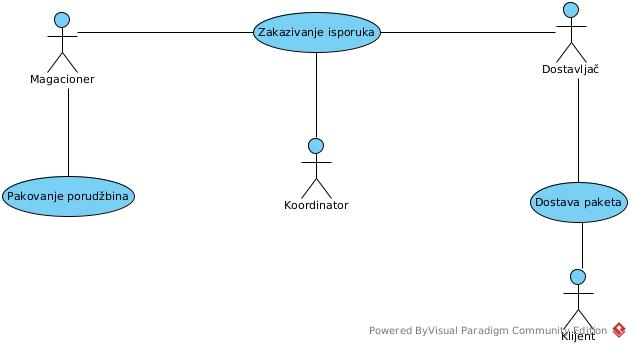
\includegraphics[width=\textwidth]{uc_delivering_package_to_customer.jpg}
	\end{center}
    \caption{Dijagram slučaja upotrebe isporučivanja paketa korisniku}
\end{figure}

Na slici 12 je prikazan dijagram sekvenci koji bi predstavio sled događaja u sistemu za 3 slučaja upotrebe: 
\begin{itemize}
	\item{Zakazivanje isporuka}
	\item{Pakovanje porudžbina }
	\item{Dostava paketa}
\end{itemize}

Koordinator je zaslužan za organizaciju dostavljača i plan isporuke paketa. Koordinator, magacioner i dostavljač mogu menjati status narudžbine i u zavisnosti od njega mogu videti da li je porudžbina upakovana ili ne, da li se porudžbina trenutno pakuje, da li je paket dostavljen ili ne. Akcije aktera u sistemu zavise od statusa narudžbina. Ceo proces se odigrava sve dok nisu isporučene sve porudžbine za narednu nedelju.


\begin{figure}[H]
	\begin{center}
		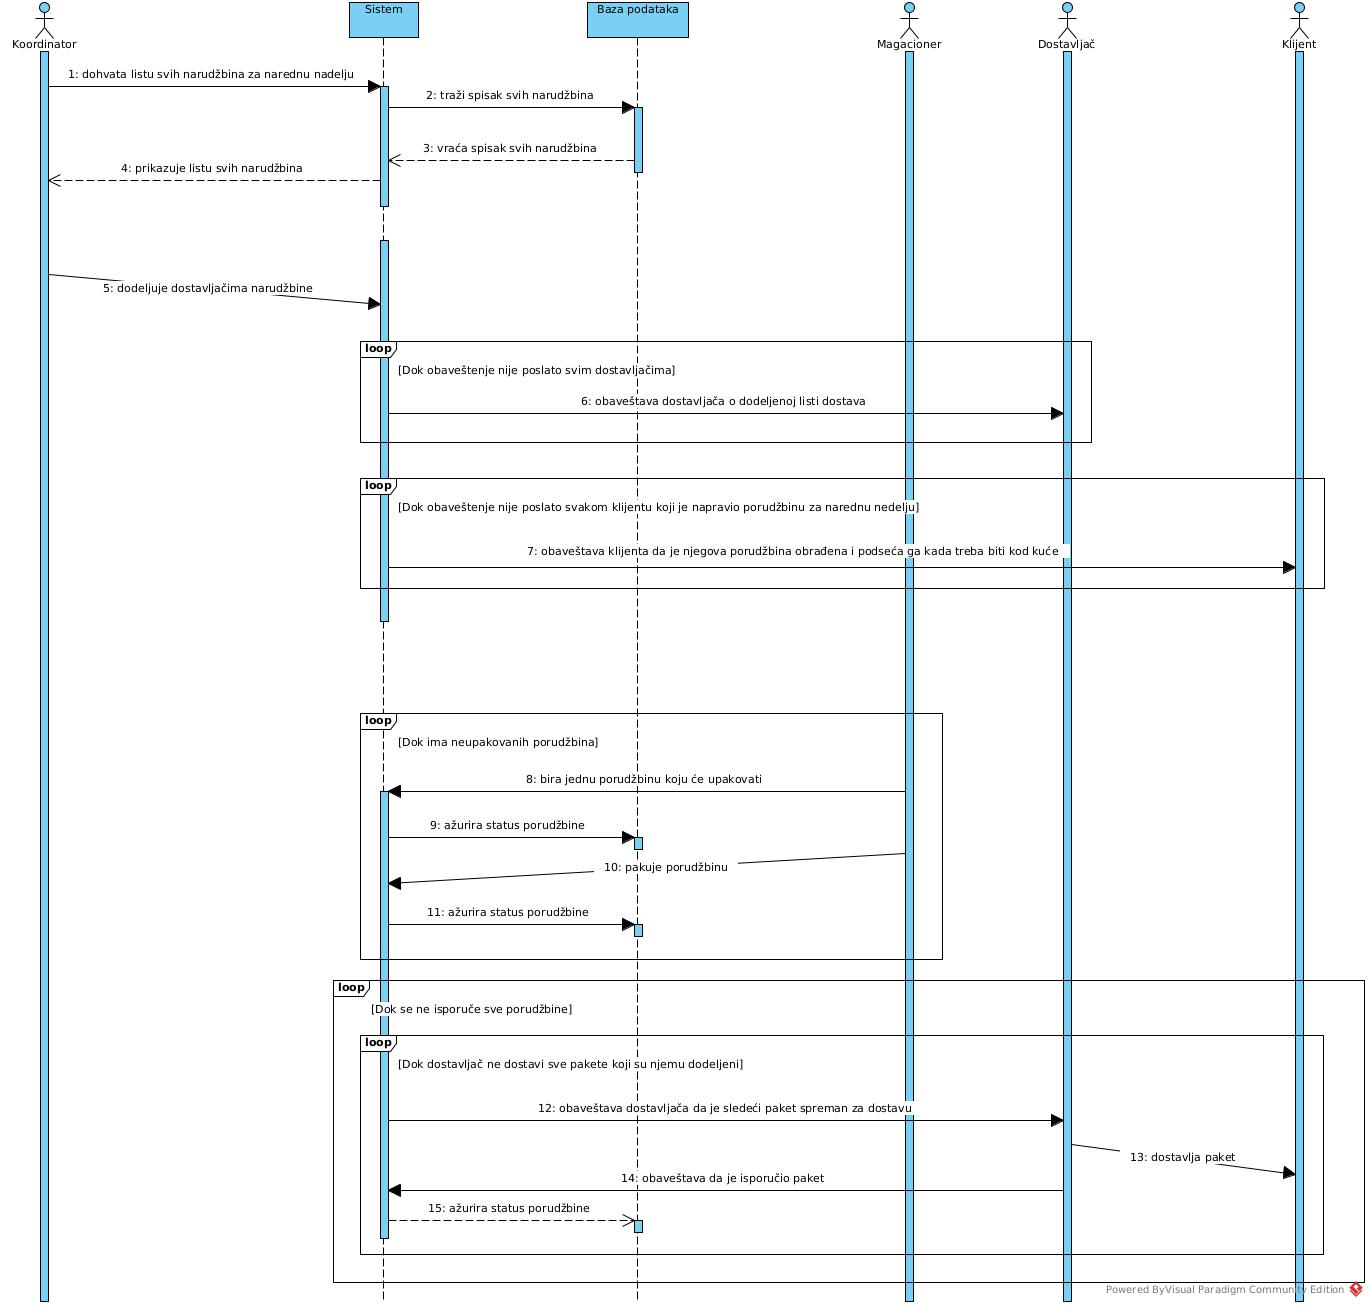
\includegraphics[width=\textwidth]{seq_delivering_packages_to_the_user.jpg}
	\end{center}
    \caption{Dijagram sekvenci isporučivanja paketa korisniku}
\end{figure}


Kroz rad sistema, poručeni paket prolazi kroz više procesa koji mu menjanju status. Na slici \ref{fig:StatePackage} je prikazan dijagram stanja paketa. 
\begin{figure}[H]
\begin{center}
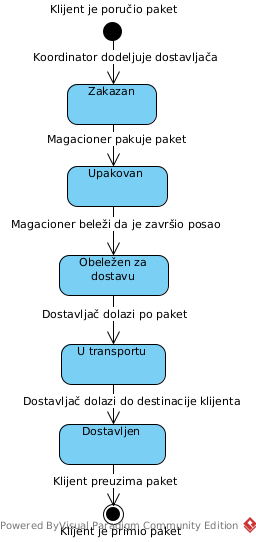
\includegraphics[scale=0.75]{Pictures/state_package.png}
\end{center}
    \caption{Dijagram stanja paketa}
\label{fig:StatePackage}
\end{figure}



\subsubsection{Zakazivanje isporuka}

\begin{itemize}
	\item Kratak opis:
		\begin{itemize}
			\item Koordinator pravi raspored dostavljačima.
		\end{itemize}
	\item Učesnici:
		\begin{itemize}
		    \item Koordinator
		\end{itemize}
	\item Preduslovi:
		\begin{itemize}
		    \item Postoji bar jedan dostupan dostavljač.
		    \item Sistem je u funkciji.
		\end{itemize}
	\item Postuslovi:
		\begin{itemize}
			\item Svaka narudžbina je dodeljena nekom od dostavljača.
	\end{itemize}
	\item Osnovni tok:
		\begin{enumerate}
            \item Koordinator pristupa sistemu i prolazi kroz sve narudžbine koje bi trebalo da se obave sledeće nedelje.
            \item Sistem pristupa bazi podataka i generiše listu svih zakazanih narudžbina za sledeću nedelju.
           \item Koordinator svakoj narudžbini dodeljuje dostavljača.
           \item Sistem svakoj narudžbini ažurira dodeljenog dostavljača.
            \item Koordinator dostavljačima preko sistema prosleđuje njegovu listu isporuka za narednu nedelju.
            \item Sistem klijentu šalje automatski mejl kojim ga obaveštava da je porudžbina obrađena i podseća  ga u koje vreme mora da bude kod kuće da bi primio porudžbinu.
		\end{enumerate}
   \item Dodatne informacije:
        \begin{itemize}
            \item Lista isporuka se sastoji od identifikacionih brojeva narudžbina, zakazanog vremena dostave i zakazanog vremena pakovanja porudžbine. 
        \end{itemize}
\end{itemize}

\begin{figure}[H]
\begin{center}
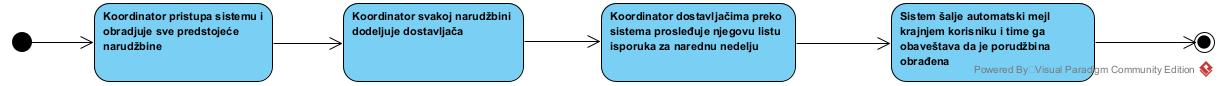
\includegraphics[width=\textwidth]{activity_diagram_scheduling_deliveries.jpg}
\end{center}
    \caption{Dijagram aktivnosti - Zakazivanje isporuka}
\label{fig:Activity_diagram_scheduling_deliveries}
\end{figure}



\subsubsection{Pakovanje porudžbina}
	\begin{itemize}
		\item{Kratak opis:} 
		
		- Magacioner pakuje porudžbine u pakete za isporuku.
		\item{Učesnici:} 
		
		- Magacioner
		\item{Preduslovi:}
		
		- Magacioner je prijavljen na sistem i ima neupakovanih porudžbina. U magacinu ima dovoljno potrebnih namirnica da se upakuju sve porudžbine.
		\item{Postuslovi:}
		
		- Nema neupakovanih porudžbina.
		\item{Osnovni tok:}
		\begin{enumerate}
			\item{Magacioner proverava listu neupakovanih porudžbina.}
			\item{Magacioner preuzima jednu porudžbinu i beleži to u sistemu.}
			\item{Magacioner pakuje paket i obeležava ga identifikacionim brojem koji dobija na osnovu sistema.}
			\item{Magacioner beleži da je završio pakovanje porudžbine i da je paket spreman za dostavu.}

			\textit{Koraci 1-4 se ponavljaju sve dok ima nedostavljenih paketa.}
		\end{enumerate}

	\end{itemize}


\subsubsection{Dostava paketa}

	\begin{itemize}
		\item{Kratak opis:} 
		\begin{itemize}
			\item{Dostavljač dobija informacije o paketu od sistema i dostavlja paket korisniku.}
		\end{itemize}
		
		\item{Učesnici:} 
		\begin{itemize}
			\item{Dostavljač, korisnik}
		\end{itemize}		
		
		\item{Preduslovi:}
		\begin{itemize}
			\item{Dostavljač je prijavljen na sistem i ima nedostavljenih paketa. }
			\item{Klijent je poručio paket.}
		\end{itemize}		

		\item{Postuslovi:}
		\begin{itemize}
			\item{Korisnik dobija svoj paket sa namirnicama.}
		\end{itemize}		
		
		\item{Osnovni tok:}
		\begin{enumerate}
			\item{Dostavljač dobija obaveštenje od sistema da ima nedostavljenih paketa.}
			\item{Dostavljač dolazi do magacina gde su smešteni paketi.}
			\item{Dostavljač očitava identifikacioni broj paketa pomoću sistema i dobija informacije o porudžbini.}
			\item{Dostavljač dolazi do destinacije korisnika u predviđenom periodu.}
			\item{Korisnik preuzima svoj paket.}
			\item{Dostavljač beleži da je uspešno izvršio dostavu.}
			
			
			\textit{Koraci 2-6 se ponavljaju sve dok ima nedostavljenih paketa.}
		\end{enumerate}
		
		\item{Alternativni tokovi:}
			\begin{enumerate}
				\item[4.a] Ukoliko dostavljač proceni da će kasniti, obaveštava korisnika pomoću sistema.
				\item[5.a] Ukoliko korisnik nije na naznačenoj adresi, dostavljač ostavlja paket ispred ulaza. Slučaj upotrebe se nastavlja od koraka 6.%Sistem obaveštava korisnika da dostavljač nije uspeo da dostavi paket i traži od korisnika da potvrdi svoju adresu. Ako je korisnik promenio adresu, sistem ga navodi na opciju ažuriranja naloga.  
			\end{enumerate}
		\item{Dodatne informacije:}
			\begin{itemize}
				\item{Spisak nedostavljenih paketa je sortiran rastuće po vremenu dostave.}
			\end{itemize}
	\end{itemize}
	
\begin{figure}[H]
	\begin{center}
		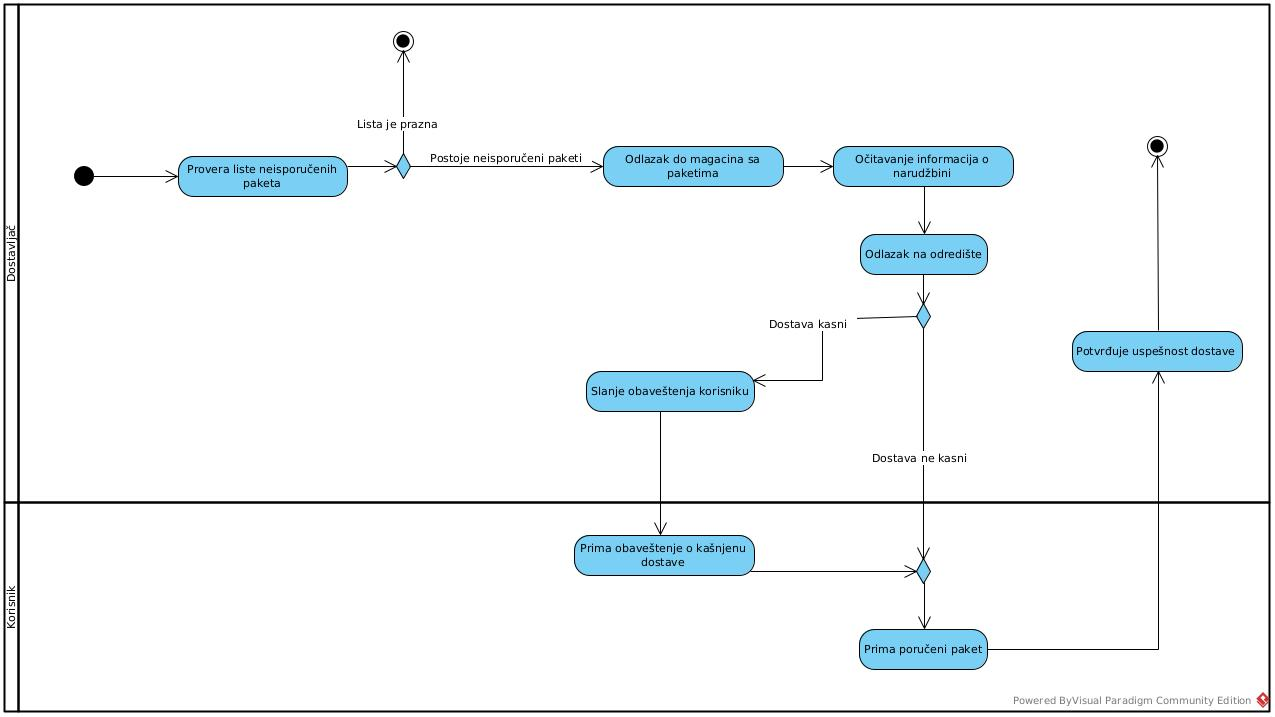
\includegraphics[width=1\textwidth]{activity_package_delivery}
	\end{center}
	\caption{Dijagram aktivnosti dostave paketa}
%	\label{fig:UCPackageDelivery}
\end{figure}	



